\documentclass[11pt]{article}
\usepackage[margin=2cm, a3paper]{geometry}                % See geometry.pdf to learn the layout options. There are lots.
%\geometry{a3paper}                   % ... or letterpaper or a4paper or a5paper or ... 
%\geometry{landscape}                % Activate for for rotated page geometry
\usepackage[usenames,dvipsnames,svgnames,table]{xcolor}
\usepackage{tikz}
\usepackage{amsmath, amssymb}
\usetikzlibrary{mindmap}
\begin{document}
\section{Partial differentiation mindmap}
\scalebox{1}{
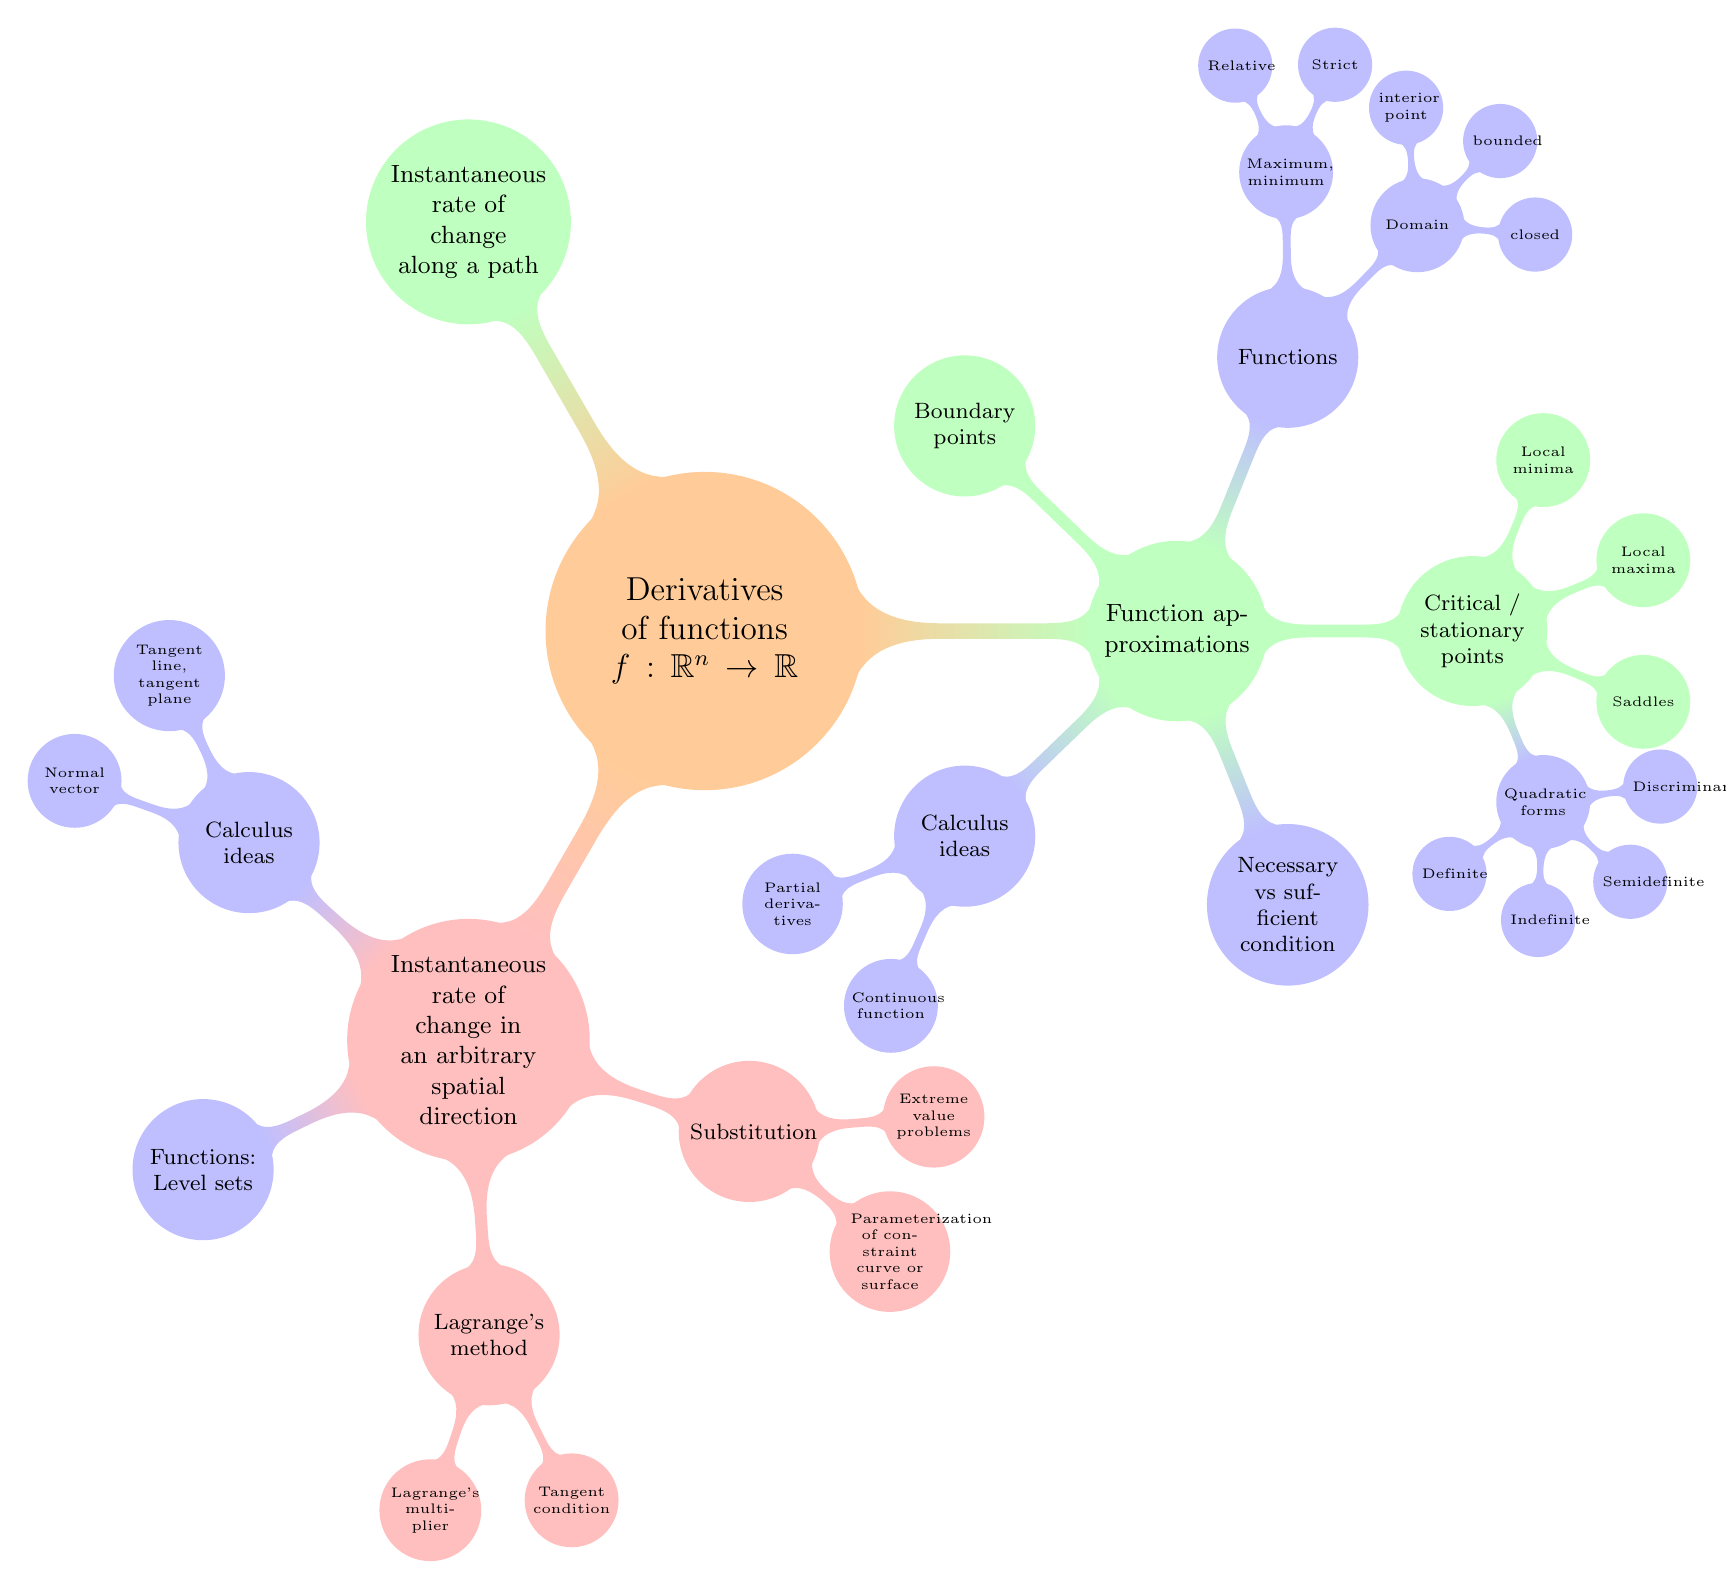
\begin{tikzpicture}[mindmap, grow cyclic, every node/.style=concept, concept color=orange!40, 
    level 1/.append style={level distance=6cm,sibling angle=120},
    level 2/.append style={level distance=3.75cm,sibling angle=68},
    level 3/.append style={level distance=2.35cm,sibling angle=45},
    level 4/.append style={level distance=1.5cm,sibling angle=50}]
    \node{Derivatives of functions $f: \mathbb{R}^n \rightarrow \mathbb{R}$}
        child[concept color=red!25] { node {Instantaneous rate of change in an arbitrary spatial direction}
          	child[concept color=blue!25]  { node {Calculus ideas}
		child { node {Tangent line, tangent plane}}
		child { node {Normal vector}}
		}
		child[concept color=blue!25] { node {Functions: Level sets}}
       	 	child { node {Lagrange's method}
			child { node {Lagrange's multiplier}}
			child { node {Tangent condition}}
		}
		child { node {Substitution}
			child { node {Parameterization of constraint curve or surface}}
			child { node {Extreme value problems}}
		}
	}
	        child[concept color=green!25] { node {Function approximations}
        child[concept color=blue!25]  { node {Calculus ideas}
		child { node {Partial derivatives}}
		child { node {Continuous function}}
		}
	child[concept color=blue!25] { node {Necessary vs sufficient condition}}
        	child { node {Critical / stationary points}
		child[concept color=blue!25] { node {Quadratic forms}
			child { node {Definite}}
			child { node {Indefinite}}
			child { node {Semidefinite}}
			child { node {Discriminant}}
		}
		child { node {Saddles}}
		child { node {Local maxima}}
		child { node {Local minima}}
		}
		child[concept color=blue!25] { node {Functions}
        		child[concept color=blue!25] { node {Domain}
			child { node {closed}}
			child { node {bounded}}
			child { node {interior point}}
		}
      		child[concept color=blue!25] { node {Maximum, minimum}
			child { node {Strict}}
			child { node {Relative}}
		}}
		child { node {Boundary points}}
		}
		 child[concept color=green!25] { node {Instantaneous rate of change along a path}};
\end{tikzpicture}
}

\end{document}
